% =============================================================================
%  Paper 2 -- target venue: Biodiversity Informatics (University of Kansas)
%  https://journals.ku.edu/jbi/index   open access, no fees, two anonymous reviews
%
%  The journal accepts Word, RTF or PDF, so this source is ours and the SUBMITTED
%  artefact is the compiled PDF. House style: double spaced, tables and figures at
%  the end on separate pages. Uncomment \doublespacing and the endfloat line below
%  for the submission build.
%
%  HOW THE NUMBERS GET HERE
%  Every table of model results is \input from generated/, written by
%      python paper2/build_results.py --part <pilot|main> --label "<run name>"
%  from the verdict rows. Re-run it after a new run and recompile; do not type a
%  model-run percentage into this file. The PROSE of Section 7.2 does quote numbers
%  from those tables and must be re-read whenever they are regenerated: it is
%  wrapped in the `prelim' environment so it is easy to find.
%
%  Anything not yet measured is tagged \pending{}. Grep for it before submitting.
% =============================================================================
\documentclass[11pt,a4paper]{article}

\usepackage[T1]{fontenc}
\usepackage[utf8]{inputenc}
\usepackage[english]{babel}
\usepackage{amsmath,amssymb}
\usepackage{graphicx}
\usepackage{booktabs}
\usepackage{tabularx}
\usepackage{microtype}
\usepackage{xcolor}
\usepackage[margin=2.5cm]{geometry}
\usepackage{setspace}
\usepackage{tikz}
\usetikzlibrary{arrows.meta,positioning}
\usepackage{natbib}
\usepackage[hidelinks]{hyperref}
\bibliographystyle{plainnat}

% Submission build:
% \doublespacing
% \usepackage[nolists,tablesfirst]{endfloat}

\emergencystretch=3em
\newcommand{\pending}[1]{\textcolor{red}{[pending: #1]}}
\newenvironment{prelim}{\par}{\par}
\newcommand{\vt}[1]{\texttt{#1}}          % verdict and question-type labels

\newcommand{\RunLabel}{20-species development run}
\newcommand{\RunSpecies}{20}
\newcommand{\RunQuestions}{238}
\newcommand{\RunAnswers}{2{,}300}


\title{\textbf{What the record can answer, and what a model merely asserts:\\
everyday questions about a tropical flora, scored against the published record}}

% Co-authors to be confirmed before submission; the companion paper's author list is
% in mpcr_rag/paper/main.tex. If the journal runs anonymous review, blank this block.
\author{José Araya Castrillo\\[2pt]
\small School of Computer Engineering, Costa Rica Institute of Technology, San José, Costa Rica\\
\small \texttt{jose2489@gmail.com}}

\date{Draft --- \today}

\begin{document}
\maketitle

\begin{abstract}
\noindent
People now ask language models where a plant grows, when it flowers and whether it
can be planted on their farm. For the regional floras of the tropics it is not known
how often the answers are true, nor whether the published record can settle the
question at all. We separate the two. On a structured catalogue of 6{,}946 species
extracted from the \emph{Manual de Plantas de Costa Rica}, a frozen and citable
download of 999{,}625 cleaned Costa Rican occurrence records, and 143 protected
areas, we first measure \emph{answerability} with no model involved: the record
settles elevation for 99.5\% of species and the slope a species grows on for 99.1\%,
whether it has been collected inside a given national park for 78.9\%, an edible or
medicinal use for 1.9\%, and a light preference for none. We then build a benchmark
of 1{,}329 everyday questions in Spanish over 117 species sampled on two popularity
axes that correlate only moderately (Spearman $\rho = 0.46$), in which every question
carries a typed answer key scoped to what the record supports. Answers are scored
without a language-model judge: deterministic parsers compare the direct answer with
the key and every individual claim with the species' full record, keeping
\emph{contradicted} apart from \emph{not in the record}. Ten conditions cross two
generators with four kinds of evidence. In a \RunSpecies-species preliminary run
(\RunAnswers{} scored answers) a frontier model answering from the serialized
evidence was correct on 46 of 48 paired questions against 23 of 48 for the same
model asked freely; the occurrence, protected-area and terrain evidence changed the
outcome only on the questions the flora does not settle; and the same model reading
the same evidence as a map was correct on 8 of 18 questions against 17 of 18 from
text, failing by caution rather than by invention. These figures are preliminary and
come from species on which the prompts were tuned; we state the confirmatory design
they motivate. Ten defects found while building the evaluation, six of which would
have produced plausible published numbers, are reported as a result in their own
right.
\end{abstract}

\noindent\textbf{Keywords:} biodiversity informatics; large language models; regional
floras; species occurrence data; answer verification; knowledge shortfalls;
abstention; Costa Rica

% =============================================================================
\section{Introduction}

Anyone with a phone can now ask a language model where a plant grows, when it
flowers, or whether it can be planted on a farm at a given altitude. The answers are
fluent and specific. Whether they are true is a separate question, and for most of
the world's plant diversity it is an open one. The accuracy of language models decays
with the popularity of the entity asked about \citep{kandpal2023longtail,
mallen2023popqa}, and a tropical regional flora consists largely of species that are
rarely collected and seldom written about outside a single published treatment.
Evaluations of ecological knowledge in these models exist, but they are closed-book
and global in scope \citep{dorm2025ecological,uryu2025iucn}. What a regional user
asks --- in Spanish, about a species known from two herbarium records --- is the
hardest case and the least measured.

Two questions are usually confounded in such evaluations, and this paper keeps them
apart.

\paragraph{Is the answer true?} This requires a model run and an answer key.

\paragraph{Could any source have answered?} This requires neither. A question is
answerable only if something in the record settles it, and for a flora that is a
countable property of the catalogue. The \emph{Manual de Plantas de Costa Rica}
\citep{hammel_manual} states an elevation range and a slope for almost every species
it treats; it almost never states whether a plant is edible, and never whether it
wants sun or shade. Occurrence records settle some of what the text leaves open, and
nothing settles the rest. Which everyday questions fall in which class is the kind of
completeness analysis that biodiversity informatics already publishes for occurrence
data \citep{arvizu2025reptiles}, applied here to questions rather than to grid cells,
and it locates the shortfalls of the record \citep{hortal2015shortfalls} in the terms
a member of the public would use.

The separation matters because the two interact. A system that answers everything
looks better than one that declines, until declining is counted as the correct
behaviour where the record is silent. An evaluation that scores silence as error
rewards invention; one that reports precision alone rewards refusing. We therefore
score what the record supports, report precision only together with coverage, and
treat a claim the record does not contain as a different thing from a claim the
record contradicts.

\paragraph{Contributions.}
\begin{enumerate}
  \item A \textbf{measurement of answerability} for a tropical regional flora: for
        each of eleven everyday question types, the fraction of 6{,}946 species the
        published record can settle and the evidence that settles it
        (Section~\ref{sec:answerability}). It requires no model and stands
        independently of everything that follows.
  \item A \textbf{benchmark with typed, record-scoped keys}: 1{,}329 questions in
        Spanish over 117 species sampled on two popularity axes, with the rule behind
        every inferred key stated and justified, including the cases in which the key
        is a rule of compatibility rather than a gold answer
        (Section~\ref{sec:benchmark}).
  \item A \textbf{two-level verification protocol with no language-model judge}, in
        which a model only segments an answer into claims and deterministic parsers
        decide every verdict (Section~\ref{sec:evaluation}).
  \item A \textbf{factorial comparison} of generator against evidence, including a
        flora-only ablation that isolates what occurrence and terrain evidence add, a
        template answerer with no model, and a within-model contrast between evidence
        delivered as text and as a map (Sections~\ref{sec:systems}
        and~\ref{sec:results}).
  \item A \textbf{defect log}: ten faults found in the evaluation itself while it was
        being built, with an account of how each was found
        (Section~\ref{sec:defects}).
\end{enumerate}

\paragraph{Status of the results.} The answerability measurement is complete. The
model comparison reported here is a preliminary run on \RunSpecies{} species,
included to fix the design and to show the direction and size of the effects; it is
not the confirmatory experiment, whose design is given in
Section~\ref{sec:confirmatory}.

% =============================================================================
\section{Related work}\label{sec:related}

\paragraph{Ecological knowledge in language models.} \citet{dorm2025ecological}
evaluate frontier models on species presence, range maps, threat classification and
trait estimation and find measurable but uneven knowledge. \citet{uryu2025iucn} tests
five models against IUCN Red List information for 21{,}955 species and reports that
taxonomic classification is far more reliable than assessment of status, with a
systematic bias toward charismatic vertebrates. Both are closed-book and global. We
test one regional flora in the language its users speak, compare grounded with
ungrounded answering on identical questions, and verify claim by claim against a
published source.

\paragraph{Long-tail knowledge and retrieval.} That models know less about rarely
mentioned entities, and that retrieval helps most exactly there, is established for
general question answering \citep{kandpal2023longtail,mallen2023popqa}; retrieval
also outperforms unsupervised fine-tuning as a way to supply specific knowledge
\citep{ovadia2024finetuning}, which is why we ground rather than fine-tune.
Retrieval-augmented generation \citep{lewis2020rag} was applied to this flora in our
earlier system \citep{araya2026grounding}, which showed that supplying the retrieved
entry raises elevation agreement from 34\% to 89\% for Costa Rican plants. That
experiment scored grounded answers against the same flora the evidence came from,
which bounds what it can claim. The present work changes the target: questions whose
keys come from occurrence data, from a stated rule over several sources, or from
nothing at all.

\paragraph{Mobilizing what is already written down.} Much of what a regional user
wants to know exists only inside documents, and recovering it is an established line
of work in this journal and elsewhere: data are rescued from environmental assessment
reports never meant as occurrence sources \citep{telletxea2026stray}, vague textual
localities are interpreted into usable geography \citep{campbell2024near}, traits are
derived automatically and anchored to the specimens that justify them
\citep{bakis2026raunkiaeran}, and language models extract occurrence and trait data
from literature and flora descriptions \citep{castro2024llm,bamba2025flora,arete2025}.
That work extracts \emph{into} the record what a text states. Trait gap-filling goes
the other way and infers unstated values statistically, with no derivation that a
reader can audit \citep{schrodt2015bhpmf}. Our target is the step after
mobilization: once the record is structured, which everyday questions can it answer,
and by what inspectable rule when the answer is not stated anywhere.

\paragraph{Verification, attribution and abstention.} Decomposing generated text into
atomic claims and checking each against a source \citep{min2023factscore}, judging
whether a statement is attributable to identified evidence \citep{rashkin2023ais},
separating truthfulness from informativeness \citep{lin2022truthfulqa,
prasad2023receval}, and representing a conclusion as premises plus inference
\citep{dalvi2021entailment} are all standard in the evaluation of language
generation. Scoring premises apart from the inference drawn from them is therefore
not new, and we do not claim it. What differs here is the setting: the target
proposition is absent from the entire corpus rather than from a retrieved passage,
the inferences that reach it are defeasible rather than deductive (a species with no
record inside a park may still grow there), and the authority is a domain record
whose silences are themselves informative. Evaluation by a language-model judge is
known to carry position, verbosity and self-enhancement biases
\citep{zheng2023judge}; our protocol avoids the judge altogether. Reporting precision
jointly with coverage follows selective prediction \citep{elyaniv2010selective,
kamath2020selective}. For biodiversity question answering specifically,
\citet{moracross2024uq} estimate when a model's answer is unreliable from the
answers alone; we measure reliability against the record instead.

% =============================================================================
\section{Data}\label{sec:data}

All components are rebuildable from citable sources, and the frozen occurrence
download fixes the evidence at a single point in time (Table~\ref{tab:data},
Fig.~\ref{fig:pipeline}).

\begin{table}[htbp]
\centering
\caption{Components of the test bed. Counts are as built and were verified against
the database on 9 October 2026.}
\label{tab:data}
\small
\begin{tabularx}{\textwidth}{lXr}
\toprule
Component & Source & Size \\
\midrule
Species catalogue      & \emph{Manual de Plantas de Costa Rica}, Vols.\ II--VI \citep{hammel_manual} & 6{,}946 species, 204 families \\
Occurrence records     & GBIF download \citep{gbif_snapshot}, cleaned & 999{,}625 records \\
Taxonomic resolution   & GBIF backbone, accepted keys & 6{,}917 species (99.6\%) \\
Protected areas        & national protected-area layer \citep{snit2024} & 143 areas \\
Species $\times$ area  & cleaned records inside protected-area polygons & 70{,}769 pairs \\
Botanical regions      & phytogeographic map of the Manual \citep{castro_regions}, digitized & 28 regions \\
Terrain                & SRTM digital elevation model \citep{farr2007srtm} & national extent \\
\bottomrule
\end{tabularx}
\end{table}

\subsection{Catalogue}
Species entries were segmented from the OCR-processed volumes and parsed into
structured fields --- elevation range with outlier bounds, slope (\emph{vertiente}),
botanical regions, forest types, growth form, flowering months and endemism ---
together with the verbatim distribution paragraph, morphological description and
taxonomic discussion. The segmentation and field extraction are those of the
companion paper \citep{araya2026grounding}, where they were developed against a
hand-checked family treatment and audited for literal textual support across the
corpus: parsed elevation bounds were attested in the source paragraph for 5{,}759 of
5{,}760 entries and every recorded slope and endemism flag matched its cue. That
audit was run on the 5{,}791 entries indexed at the time. The catalogue used here
holds 6{,}946. \pending{state what was added between the two papers and re-run the
audit on the 6{,}946 entries, so the support figures apply to this catalogue.} The
fields are produced deterministically, so each value can be traced to the sentence
that produced it. Two fields of the schema, global range and uses, are not extracted;
Section~\ref{sec:keys} explains how the two question types that would have read them
are keyed instead.

\subsection{Occurrence evidence}
Records were cleaned with the rules of the companion paper's mapping pipeline:
accepted taxon keys only, coordinates inside the national bounding box, swapped
latitude and longitude repaired, and records with coordinate uncertainty above 10~km
discarded, following standard practice for collection data
\citep{zizka2019coordinatecleaner}. Each record carries an elevation sampled from the
digital elevation model, the botanical region it falls in, and a 30-arc-second cell
identifier used to count distinct collection sites rather than duplicate records. Per
species we aggregate record counts, distinct sites, regions, and the protected areas
the records fall within. Occurrence data of this kind reflect where collectors went
as much as where plants grow \citep{beck2014spatial,meyer2016multidimensional}. Every
rule in Section~\ref{sec:keys} that reads these records is written with that in mind.

\subsection{Protected areas, regions and terrain}
For each of the 143 terrestrial protected areas we compute at build time the
botanical regions it intersects and the 5th and 95th percentiles of elevation inside
its polygon, and for each species the number of cleaned records inside it, in total
and since 1970. These are stored as facts. No system in the experiment performs a
spatial computation: by the time a model sees a question, ``two records inside the
park since 1970; park elevation 300--900~m; regions shared: one'' is a row and not an
inference. This is a design decision and Section~\ref{sec:systems} returns to it.

\begin{figure}[htbp]
\centering
\resizebox{\textwidth}{!}{%
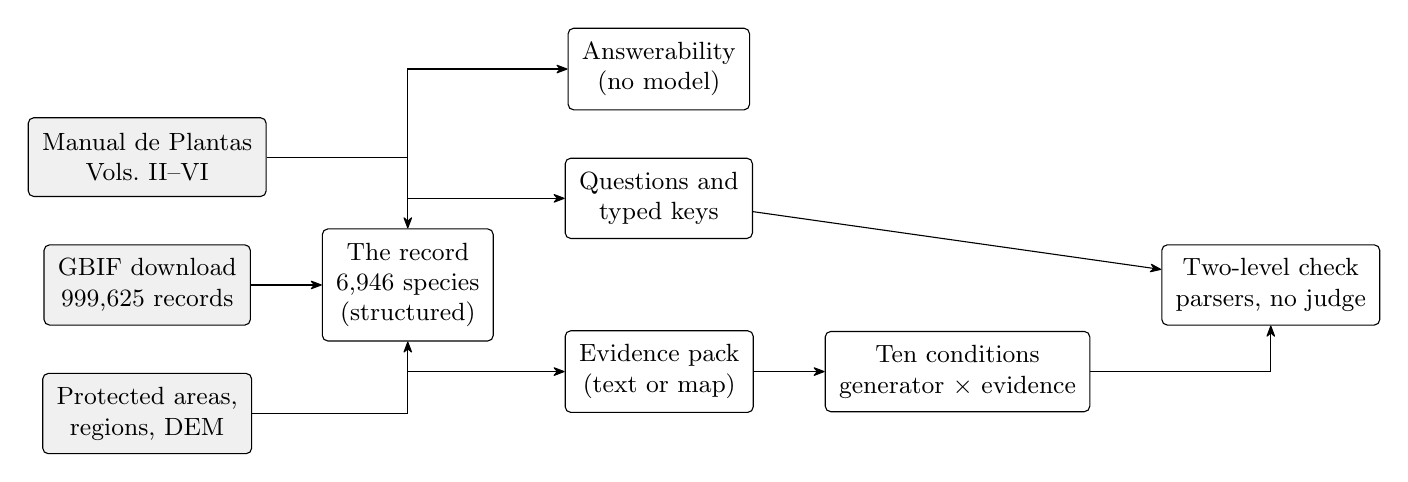
\begin{tikzpicture}[>={Stealth[round]}, node distance=6mm and 9mm,
  box/.style={draw, rounded corners=2pt, align=center, font=\small, inner sep=5pt,
              minimum height=10mm},
  src/.style={box, fill=black!6}]
\node[src] (man) {Manual de Plantas\\Vols.\ II--VI};
\node[src, below=of man] (gbif) {GBIF download\\999{,}625 records};
\node[src, below=of gbif] (geo) {Protected areas,\\regions, DEM};
\node[box, right=of gbif] (rec) {The record\\6{,}946 species\\(structured)};
\node[box, right=of rec, yshift=11mm] (keys) {Questions and\\typed keys};
\node[box, right=of rec, yshift=-11mm] (pack) {Evidence pack\\(text or map)};
\node[box, right=of pack] (arms) {Ten conditions\\generator $\times$ evidence};
\node[box, right=of arms, yshift=11mm] (ver) {Two-level check\\parsers, no judge};
\node[box, above=of keys] (ans) {Answerability\\(no model)};
\draw[->] (man) -| (rec);
\draw[->] (gbif) -- (rec);
\draw[->] (geo) -| (rec);
\draw[->] (rec) |- (keys);
\draw[->] (rec) |- (pack);
\draw[->] (rec) |- (ans);
\draw[->] (pack) -- (arms);
\draw[->] (arms) -| (ver);
\draw[->] (keys) -- (ver);
\end{tikzpicture}}
\caption{The test bed. Three citable sources are structured into one record. The
record alone yields the answerability measurement; it also yields the question keys
and, separately, the evidence shown to each condition. Answers are checked against
the keys and against the full record by deterministic parsers.}
\label{fig:pipeline}
\end{figure}

% =============================================================================
\section{Benchmark}\label{sec:benchmark}

\subsection{Species sampling}\label{sec:sampling}
Two notions of ``rare'' are usually conflated. A species may be globally familiar and
locally scarce --- \emph{Stellaria media} has 821{,}441 occurrence records worldwide
and two in Costa Rica --- or locally well collected and globally obscure. We measure
both: $G$, the number of GBIF occurrence records worldwide for the accepted taxon
(retrieved 13 September 2026), and $L$, the number of records in the frozen Costa
Rican download. Over the 6{,}917 species with an accepted key the two correlate only
moderately (Spearman $\rho = 0.46$). They also drive different hypotheses: what a
model has seen in training should follow $G$ \citep{kandpal2023longtail}, whereas
what the record can confirm follows $L$.

The sampling frame is the catalogue minus three groups, each counted: 28 unnamed
morphospecies, which cannot be asked about by name; one species with no accepted key;
and 136 species whose accepted key is shared with another catalogue entry, where the
Manual separates what the backbone lumps and occurrence evidence cannot be attributed
to either. This leaves 6{,}781 species. The frame is cut at the tertiles of $G$ (149
and 986 records) and of $L$ (20 and 78 records) into nine cells, and species are
drawn with \emph{equal allocation per cell}, so that the off-diagonal cells are as
well represented as the diagonal although they are much smaller in the frame (the
cell of globally obscure, locally well-collected species holds 109 species; the cell
obscure on both axes holds 1{,}272). Estimates for the flora as a whole must
therefore be reweighted by the frame size of each cell, which the sample file
records. Two species per cell form a pilot sample ($n = 18$) and eleven per cell the
main sample ($n = 99$); the two are disjoint and frozen with a recorded seed.

\subsection{Question types}
Questions are posed in Spanish, in the form a visitor, grower or naturalist would
use, and are generated from templates so that the wording is identical across
species. There are twelve types (Table~\ref{tab:questions}): 208 questions over the
pilot species and 1{,}121 over the main sample. A type is generated for a species
only when its key exists, which is why the counts per type differ.

\begin{table}[htbp]
\centering
\caption{Question types, with the number generated for the main sample of 99 species,
the basis of the key, and its evidence level. \emph{Stated}: the flora says it.
\emph{Records}: occurrence records show it. \emph{Rule}: derived by a stated rule
from several sources. \emph{None}: the record is silent and declining is the correct
answer.}
\label{tab:questions}
\small
\begin{tabularx}{\textwidth}{lrXl}
\toprule
Type & $n$ & Question (translated) and basis of the key & Level \\
\midrule
\vt{elevation}       & 98 & ``At what altitude does it grow?'' Flora range, with outlier bounds. & stated \\
\vt{vertiente}       & 98 & ``Caribbean slope, Pacific, or both?'' Flora. & stated \\
\vt{flowering}       & 97 & ``In which months does it flower?'' Flora. & stated \\
\vt{endemism}        & 98 & ``Is it endemic to Costa Rica?'' Flora marker, or a stated range beyond the country. & stated \\
\vt{growth\_form}    & 82 & ``Tree, shrub, herb, epiphyte or vine?'' Species description, else an unambiguous genus. & stated / relatives \\
\vt{park\_confirmed} & 78 & ``If I visit park $P$, can I find it?'' At least one record inside $P$ since 1970. & records \\
\vt{park\_possible}  & 93 & Same question. No records in $P$; regions and elevation both overlap. & rule \\
\vt{park\_unlikely}  & 85 & Same question. No records in $P$; neither overlaps. & rule \\
\vt{cultivation}     & 98 & ``My farm is in $S$ at about $e$~m. Could I plant it?'' Elevation and slope of $S$ against the natural range. & rule \\
\vt{co\_occurrence}  & 96 & ``What other plants might I see at the same site?'' Compatibility of each species named. & rule \\
\vt{outside\_record} & 99 & ``Is it edible or medicinal?'' Whatever the entry states; usually nothing. & stated / none \\
\vt{light}           & 99 & ``Full sun or shade?'' No source; awaiting expert labels. & pending \\
\bottomrule
\end{tabularx}
\end{table}

\subsection{What a key is, and the rules behind the inferred ones}\label{sec:keys}

\paragraph{Keys describe the record, not the field.} Every key carries an explicit
scope: it is the answer that the published flora and the frozen occurrence download
support. A species may well grow somewhere neither mentions, and for a cosmopolitan
weed collected twice in the country that is likely. The key is still correct about
the record, and an evaluation against it measures agreement with the record. We make
no stronger claim, and Section~\ref{sec:limits} discusses what follows.

Seven types are lookups of a stated field. The other five apply a rule, and since a
rule is where a key can be wrong, each is given with its reason.

\paragraph{Protected areas: three questions from one template.} The candidate areas
are national parks and biological reserves that have an elevation profile and are not
mostly marine. For a species and a park we know the records inside the polygon,
whether the park's botanical regions intersect the species' regions, and whether the
park's elevation span (5th to 95th percentile) overlaps the species' elevation range
including outlier bounds. The key is \emph{yes} when at least one record lies inside
since 1970; \emph{possible} when there are no records at all but regions and
elevation both overlap; and \emph{unlikely} when there are no records and neither
overlaps. A park that satisfies one overlap and not the other is not used for that
species, because an ambiguous key scores noise. One park of each kind is drawn per
species where one exists, so that a yes-or-no question is never trivially ``yes''.

The rule deliberately refuses to read an absence of records as absence of the
species. Collection effort is uneven \citep{beck2014spatial,
meyer2016multidimensional}, so for a park that overlaps a species' range and holds no
record of it, \emph{possible} is the verdict the evidence supports. The 1970 cut-off
for a confirming record is a judgement about how old a record may be and still
indicate presence; its effect on the keys has not been measured
(Section~\ref{sec:limits}).

\paragraph{What counts as a species' range.} A species' regions are those the Manual
lists together with any region holding at least five cleaned records. The threshold
is the one already used by the distribution-map renderer of the companion paper,
which two specialists in the Costa Rican flora reviewed against expert reference maps
\citep{araya2026grounding}; we adopt it rather than introduce a second one. The need
is concrete. \emph{Anthurium ravenii} is listed by the Manual from four Caribbean
lowland regions, while 103 of its records lie in the Osa Peninsula; keying a park
there as \emph{unlikely} would key against the evidence. Fifty of the 117 sampled
species gain at least one region this way, and ten of 300 park questions change key.

The principle behind this is that \emph{occurrence evidence may extend a stated fact
and may not overrule one}. Regions are additive: ``also here'' does not contradict
``here'', so the union is coherent. Elevation is not. For \emph{Cryptocentrum flavum}
the Manual gives 950--1050~m and the records span 423--1248~m; two ranges cannot both
be the answer to ``at what altitude does it grow'', so the Manual's stands as the key
and the competing range is withheld from the evidence shown to the systems. Without
that, the comparison would measure which source a model privileges rather than
whether it answers truthfully. A single definition of the range is read by the keys,
the evidence pack, the map stimulus and the co-occurrence check, so that a key and
the evidence it is scored against cannot drift apart.

\paragraph{Cultivation.} The question names one of eleven real settings with its
elevation, from Puntarenas at 10~m to the slopes of Volcán Irazú at 2{,}800~m, each on
a known slope. The key is \emph{likely} when the site's elevation lies inside the
Manual's core range and the slope matches; \emph{uncertain} when it lies only inside
the outlier range, or inside the core range on the other slope; and \emph{unlikely}
otherwise. The key states its own limit: growing a plant outside its natural range
under cultivation is not tested, and an answer that says so is not marked wrong.
Whether a slope mismatch should downgrade an in-range elevation is a botanical
judgement on which we have not yet obtained an expert opinion.

\paragraph{Growth form.} The key is read from the opening of the species' own
description, with a default for families of uniform habit. Only when that yields
nothing does it fall back to the genus description, and only when the genus names a
single growth form. Genus descriptions list every form found in the genus, and
without that restriction \emph{Stellaria media}, a chickweed, was keyed as a vine and
an epiphyte. Eight of the 82 main-sample keys rest on the genus and are labelled as
inferred from relatives.

\paragraph{Endemism.} The key reads the Manual's endemism marker, or else looks in
the range statement that closes the distribution paragraph for territory beyond Costa
Rica. One or the other is present for 98.4\% of species.

\paragraph{Edible or medicinal use.} The question asks specifically whether a plant
is edible or medicinal, so its key turns on a mention of edibility or medicine in the
entry and not on a mention of any use. This distinction was learned from an error
(Section~\ref{sec:defects}): keyed on any use, \emph{Dalbergia retusa} counted as
having a stated use because its entry mentions timber, and a system that correctly
declined to call it edible was marked as understating. For the 97 of 99 main-sample
species whose entry mentions neither, the key is that the record is silent and the
correct response is to say so.

\paragraph{Co-occurrence: compatibility, not a gold list.} ``If I find $X$ in the
field, what other plants might I see at the same site?'' has no usable gold answer.
The species that share a botanical region and an overlapping elevation band with a
given species number between 1{,}900 and 3{,}200, about a third of the flora, and
occurrence data do not narrow this, because the species co-recorded in the same grid
cells number 1{,}200 to 2{,}500. Almost any real Costa Rican plant would be scored
correct. The key therefore inverts: it does not ask whether a named plant is on a
list but whether it is possible at all, that is, whether it shares a region and an
elevation band with the subject. Co-occurrence is common; incompatibility is rare
and mechanical to detect. The question is scored on precision over what the answer
volunteers and never on recall.

Each species an answer names is resolved, synonyms first, into one of three tiers. It
is \emph{assessable} if it is in the catalogue with regions and elevation, and its
compatibility is then decided. It is \emph{outside scope} if it is absent from the
catalogue but recorded in Costa Rica in the occurrence download, which holds
13{,}504 species; such a name is not held against the answer. It is
\emph{unrecognised} if it appears in neither, which is reported and never called a
fabrication. The middle tier exists because the ingested volumes are not the whole
flora: \emph{Rhizophora mangle}, a common mangrove, is absent from them, as is every
fern. The subject species is excluded from its own list of neighbours.

\paragraph{Types without a key.} Light preference is stated for none of the 6{,}946
species. The type is generated, answered and stored, but not scored; it becomes
scoreable only with expert labels. It is in the benchmark because a question that no
source can settle is the direct test of whether a system knows to stop.

% =============================================================================
\section{Conditions compared}\label{sec:systems}

The comparison is a two-factor design, generator crossed with evidence, rather than a
list of named systems, so that any two cells differ in a stated respect
(Table~\ref{tab:design}).

\begin{table}[htbp]
\centering
\caption{Design. Rows vary the generator, columns the evidence it may use. Letters
are the condition labels used throughout. Closed-book conditions are run under two
prompts, careful and free (Section~\ref{sec:prompts}).}
\label{tab:design}
\small
\begin{tabular}{lcccc}
\toprule
Generator & no evidence & flora text only & full evidence pack & map only \\
\midrule
Frontier model (Mistral Large 4)   & A1, A1F & E  & D & DM \\
Open weights (Gemma 4 31B)         & C, CF   & -- & F & FM \\
Template, no model                 & --      & -- & G & -- \\
\bottomrule
\end{tabular}
\end{table}

\subsection{The evidence pack}
For a species and a question type the pack assembles what the record holds that bears
on the question, serialized as short labelled blocks of Spanish text with the source
of each. It exists at two levels: \emph{flora}, the Manual entry alone, and
\emph{full}, which adds occurrence, protected-area, region and terrain evidence. The
difference between the two is exactly what condition E removes. Three properties are
deliberate.

\emph{No model reasons spatially.} Region overlap, elevation overlap and counts of
records inside a polygon are computed when the pack is built and written as facts.
For the park questions the grounded conditions are therefore handed the inputs to
the key's own rule, and their score there measures faithful use of computed evidence,
not spatial inference. We state this plainly because it is the claim the design
makes: a spatial relation that a model reads off a figure sits in the one component
that cannot be verified, and Section~\ref{sec:map} tests that alternative directly.

\emph{Occurrence evidence fills gaps and does not compete with a stated fact.} For a
question whose key is a stated Manual fact, occurrence evidence enters the pack only
where the Manual is silent (Section~\ref{sec:keys}). In consequence D and E receive
identical evidence on the Manual-stated types and differ only on the park types and,
through record-derived regions, on slope. The ablation is therefore pre-specified on
the park questions; averaged over all questions it would be diluted by the questions
on which the two conditions cannot differ.

\emph{The pack never states what to answer.} Where the record is silent the pack
simply lacks the fact. It carries no sentence saying that the record is silent,
because that would hand the grounded conditions the abstention the experiment is
trying to measure. It does carry, for a park with overlap and no records, the
sentence that uneven collection effort means absence of records is not evidence of
absence. That is a property of the evidence and not an instruction about the answer.

The median full pack is 781 characters and the 90th percentile 1{,}820, small enough
for a model with a short context window.

\subsection{Prompts}\label{sec:prompts}
Every model condition that receives evidence, and the careful closed-book conditions,
share one system prompt; an arm either appends an evidence section to the user
message or does not, and nothing else varies. The harness asserts that their template
hashes are equal before it will start a run. The shared prompt licenses declining in
identical words for every condition, since licensing it only where evidence is
supplied would make any comparison of abstention an artefact of the prompt.

The shared prompt tells a model to say so when it lacks a basis to answer and not to
invent place names, elevations, months or uses. With an evidence section in front of
it that is a faithfulness instruction. With none, it is close to an instruction not
to answer, since the questions ask for exactly those things. We therefore run each
closed-book generator under a second, \emph{free} prompt that keeps the role, the
language and the length and removes the cautions (conditions A1F and CF). This is
what a person gets by simply asking, and it is the condition in which invention can
be observed at all. Both families are reported, and each answer row records which it
used.

\subsection{Evidence as a map}\label{sec:map}
Conditions DM and FM receive the question and a map, and no text evidence. The map is
rendered for the question: it shows the species' cleaned records, the botanical
regions of its range, the ground inside its elevation band within those regions, and
the asked-about park outlined and named (Fig.~\ref{fig:qmap}). It is a separate
renderer from the expert-facing map of the companion paper, for a reason found by
inspection: that map does not draw the park a question asks about, and its legend
names the slope and regions, which prints the answer to two question types on the
image. The stimulus map carries what the text pack carries and nothing a key turns
on. The condition applies only to the four types whose answer turns on geometry: the
three park types and slope.

The same two generators read the map and read the pack, so the contrast is within
model. It is not a fair fight and is not presented as one: the map is rendered from
the pack and cannot contain more. It is a ceiling check on the alternative design in
which a multimodal model reads a distribution map directly.

\begin{figure}[htbp]
\centering
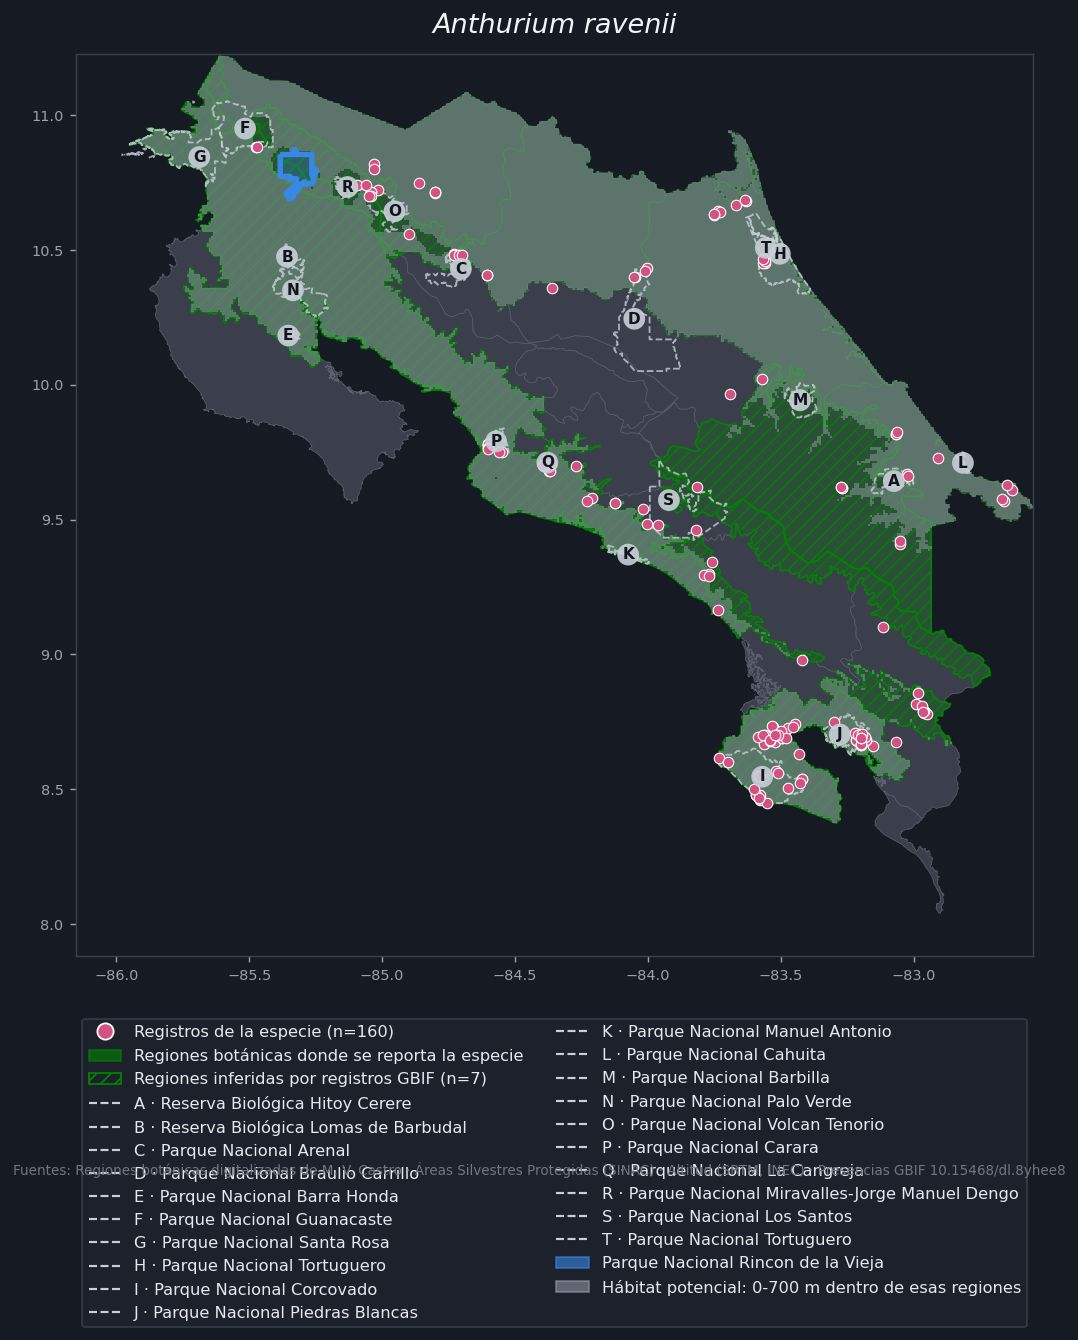
\includegraphics[width=0.62\textwidth]{figs/example_qmap.png}
\caption{A map stimulus, for ``If I visit Parque Nacional Rincón de la Vieja, can I
find \emph{Anthurium ravenii}?'' The key is \emph{possible}: no record lies inside
the park (outlined in blue), while the park overlaps the species' regions and
elevation band. Records are the pink points; hatched regions are those added by the
five-record rule. \pending{replace with a light-background render for print, and fix
the source line that overlaps the legend.}}
\label{fig:qmap}
\end{figure}

\subsection{The template condition}
Condition G uses no model. It implements each key's rule over the structured facts of
the same pack and prints a Spanish sentence with the source. It serves two purposes
and its score must be read accordingly: it is a consistency check between the keys
and the evidence, and an upper bound on what the evidence layer can deliver. Because
it applies the key's rule to the key's inputs, a perfect score for G is expected and
is not evidence that the task is easy.

\subsection{Models and reproducibility}
The frontier generator is \texttt{mistralai/mistral-large-4-0} and the open-weights
generator \texttt{google/gemma-4-31b-it}, both called through the OpenRouter API at
temperature zero with a fixed seed and a completion budget of 1{,}400 tokens. They
were chosen on three grounds: both accept a temperature and a seed, which several
current flagship models do not; they come from different vendors, so a closed-book
result is not a property of one company's training data; and both accept images, so
the map contrast is within model. One of the two has downloadable weights, which
makes two rows of the design reproducible without a proprietary service.

A routed API is not a model. The open-weights identifier is served by more than a
dozen upstream providers at different numeric precisions, and an unpinned request may
be answered by any of them. Each request therefore pins the upstream and forbids
fallback, and each answer row records the upstream that served it; a row where the
two disagree is discarded. In the runs reported here the pin held on every call.
\pending{The open-weights pin currently admits two upstreams, Crusoe and Novita, and
most calls were served by the second; confirm that both serve unquantized weights or
restrict the pin to one before the confirmatory run.} A blank completion is recorded
as an error and retried, never as an answer, because the frontier generator spends
most of a short completion on hidden reasoning tokens and an empty answer would
otherwise be scored as an abstention. Metered cost over the preliminary run was
US\$0.57 for 412 model calls.

A web-search condition was designed and is not run. The API no longer exposes
search-enabled model identifiers, so search is a request-time plugin whose backend
would become part of the system under test; until that backend can be named and its
retrieved pages logged, the condition would not be reproducible.

% =============================================================================
\section{Evaluation}\label{sec:evaluation}

\subsection{Two levels, and no judge}
Each answer is scored at two levels. \emph{Level 1} compares the direct answer with
the question's key. \emph{Level 2} compares every factual claim the answer makes
along the way with the species' full record, not only with the key.

No language model assigns a verdict. A local model that is neither generator
(\texttt{qwen3-vl:8b-instruct}, run through Ollama at temperature zero) reads the
answer and returns three things: whether it declines, its stance on a yes-or-no
question (yes, possible, no, uncertain), and the answer split into typed claims. From
there everything is deterministic. Elevations, months, slopes and growth forms are
parsed by regular expressions from the text of the answer or claim, never taken from
the model's output, and compared with stored values; a stance is mapped to a verdict
by a fixed table per key value (Table~\ref{tab:verdicts}). The model segments; it
does not adjudicate. This removes the objections that attach to a language-model
judge \citep{zheng2023judge} --- which the companion paper had to guard against with
an ensemble and a self-preference filter --- at the price of a segmentation step
that must itself be validated (Section~\ref{sec:checker}).

\begin{table}[htbp]
\centering
\caption{Verdict vocabulary.}
\label{tab:verdicts}
\small
\begin{tabularx}{\textwidth}{llX}
\toprule
Level & Verdict & Meaning \\
\midrule
Direct & \vt{correct}            & matches the key within tolerance \\
       & \vt{partially\_correct} & overlaps the key but extends beyond it or omits part of it \\
       & \vt{overstated}         & asserts more certainty than the record supports (``yes'' where the key is \emph{possible}) \\
       & \vt{understated}        & hedges where the record is definite (``possible'' where records confirm) \\
       & \vt{wrong}              & contradicts the key \\
       & \vt{abstained}          & declines on a question the record settles \\
       & \vt{beyond\_record}     & asserts something on which the record is silent; left to expert adjudication \\
       & \vt{not\_scored}        & no key exists yet (light) \\
\midrule
Claim  & \vt{supported}          & the record states it, or records show it \\
       & \vt{contradicted}       & the record states otherwise \\
       & \vt{not\_in\_record}    & checkable, but the record does not contain it \\
       & \vt{unverifiable}       & no source in the record covers this kind of claim \\
\bottomrule
\end{tabularx}
\end{table}

Three tolerances are set by judgement and stated here so they can be challenged. An
elevation is compared with a margin of 200~m. A flowering answer is \vt{correct} when
at least three quarters of the months it names are in the key and it names at least
half of the key's months, and \vt{wrong} when fewer than a quarter are. A slope
answer must equal the key's set exactly to be \vt{correct}.

The distinction between \vt{contradicted} and \vt{not\_in\_record} carries the
scientific weight of the protocol. A region the Manual does not list and in which no
record falls is not thereby a region where the species is absent, and a true
statement the flora happens not to contain --- a widely known forage use of a pasture
grass --- is not thereby false. The first is \vt{not\_in\_record}; the second is
\vt{beyond\_record} at level 1 and \vt{unverifiable} at level 2, and only a botanist
can separate knowledge the record lacks from invention.

On a question where the record is silent, an answer that declines, or that correctly
denies that the record mentions a use, is scored \vt{correct}.

\subsection{Metrics}
Four quantities are reported together and none alone.
\begin{itemize}
  \item \textbf{Precision when answering}: \vt{correct} answers over answered
        scoreable questions, where answered excludes \vt{abstained}.
  \item \textbf{Coverage}: answered over scoreable questions. Scoreable excludes
        \vt{not\_scored} and \vt{beyond\_record}.
  \item \textbf{Contradiction rate}: \vt{contradicted} claims over all claims.
  \item \textbf{Correct silence}: on questions the record cannot settle, the share
        answered by declining or by denying, against the share that assert a use.
\end{itemize}
Precision and coverage are reported as a pair because each alone can be gamed: a
system that declines everything has perfect precision and no coverage, and one that
always guesses has the reverse \citep{elyaniv2010selective}. Note that a correct
silence counts as an answered, correct question under these definitions, so a system
that declines everything still shows nonzero coverage from the silent questions
alone. We keep the definition because it is the one the harness implements, and we
report the silent questions separately so the effect is visible; the confirmatory
analysis reports precision and coverage both with and without them.

Proportions carry Wilson 95\% intervals \citep{wilson1927}. Contrasts between
conditions are paired on the question: an observation is 1 when the direct verdict is
\vt{correct} and 0 otherwise, abstentions included, over questions scoreable in both
conditions, and the test is McNemar's \citep{mcnemar1947} in its exact binomial form
on the discordant pairs.

\subsection{Validating the checker}\label{sec:checker}
The checker reproduces 24 of 24 direct verdicts on hand-written answers spanning
correct, wrong, overextended, overconfident, hedged, declining and invented
responses, and detects 12 of 12 planted false claims. Those answers were written by
the author and are cleaner than model output, so this establishes that the rules are
implemented as intended and nothing more. \pending{Agreement between the checker and
a human on 40 answers sampled from the free closed-book conditions, as a confusion
matrix. This is the measurement that licenses every model-run number in the paper and
it must precede the confirmatory run.} Section~\ref{sec:defects} explains why we rank
this above every other outstanding item.

% =============================================================================
\section{Results}\label{sec:results}

\subsection{Answerability}\label{sec:answerability}
Table~\ref{tab:answerability} and Fig.~\ref{fig:answerability} give, for each
question type, the number of species for which the record settles the question. The
predicates are those that generate the benchmark's keys, imported rather than
reimplemented, so the table describes the benchmark that exists. Two denominators are
used: the catalogue (6{,}946) for the types the Manual settles, and the species with
an accepted taxon key (6{,}917), to which occurrence evidence can be attributed, for
the park types.

\begin{table}[htbp]
\centering
\caption{Answerability across the whole catalogue. No model is involved.}
\label{tab:answerability}
\small
\begin{tabular}{lrrrl}
\toprule
Question type & Settled & Of & \% & Settled by \\
\midrule
elevation & 6{,}912 & 6{,}946 & 99.5 & Manual elevation range \\
cultivation & 6{,}912 & 6{,}946 & 99.5 & Manual elevation and slope \\
vertiente & 6{,}883 & 6{,}946 & 99.1 & Manual slope statement \\
endemism & 6{,}838 & 6{,}946 & 98.4 & ENDEMICA, or a range beyond Costa Rica \\
flowering & 6{,}626 & 6{,}946 & 95.4 & Manual phenology \\
park\_possible & 6{,}209 & 6{,}917 & 89.8 & region and elevation overlap, no records \\
park\_unlikely & 5{,}873 & 6{,}917 & 84.9 & no region overlap, no elevation overlap, no records \\
growth\_form & 5{,}855 & 6{,}946 & 84.3 & species description, else an unambiguous genus \\
park\_confirmed & 5{,}458 & 6{,}917 & 78.9 & records inside the polygon since 1970 \\
any use mentioned & 249 & 6{,}946 & 3.6 & a use named in the Manual text \\
edible or medicinal use & 133 & 6{,}946 & 1.9 & an edible or medicinal use named in the entry \\
light & 0 & 6{,}946 & 0.0 & nothing in the record \\
\bottomrule
\end{tabular}

\end{table}

\begin{figure}[htbp]
\centering
\includegraphics[width=0.78\textwidth]{figs/fig_answerability.pdf}
\caption{Share of species for which the record settles each question type.}
\label{fig:answerability}
\end{figure}

The record divides sharply. It settles where a plant grows --- its elevation, its
slope, whether it is endemic --- for more than 98\% of species, and when it flowers
for 95.4\%. It settles what the plant looks like at the coarsest level, its growth
form, for 84.3\%, of which 824 species only by an unambiguous genus. For 78.9\% of
species at least one national park or biological reserve holds a record since 1970.
It settles what a plant is good for almost never. Counting the Manual's own use
vocabulary finds a mention of any use (timber, ornament, cultivation, toxicity,
food, medicine) in 249 entries, 3.6\%, and a mention of an edible or medicinal use in
133, 1.9\%. The two figures measure different things and both are reported: the first
is the Manual's coverage of use in general, the second the answerability of the
question a person actually asks. Light preference is stated for no species.

This is not a criticism of the Manual, which is a taxonomic treatment and does what
such a treatment is for. It is a description of what a system grounded in it can and
cannot say, with two consequences for evaluation. A benchmark built only from
elevation, slope and phenology would be answerable for nearly every species, would
put every grounded system at ceiling, and would never observe a system at the edge of
its evidence. And for the commonest practical questions about a plant --- can I eat
it, will it cure something, where should I put it in my garden --- the correct
behaviour of a system grounded in the published flora is, for 98 species in 100, to
say that the record does not say.

\subsection{Preliminary model comparison}\label{sec:prelim}

\begin{prelim}
\emph{The numbers in this subsection come from the \RunLabel: \RunSpecies{} species,
\RunQuestions{} questions and \RunAnswers{} scored answers. The five species are
pilot species on which prompts and scoring rules were tuned (}Aspidosperma cruentum,
Clethra consimilis, Clidemia gracilis, Cryptocentrum flavum \emph{and} Phaseolus
talamancensis\emph{, covering five of the nine sampling cells). They show direction
and rough size. Intervals are wide, tests are unadjusted, and nothing here is a
confirmatory result.} \pending{Replace with the 20-species run when it is scored, by
re-running \texttt{build\_results.py}; then re-read every number quoted in this
subsection against the regenerated tables.}

\begin{table}[htbp]
\centering
\caption{Conditions in the \RunLabel. $n$: scoreable questions. Precision is over
answered questions; the interval is Wilson 95\%. Coverage is answered over scoreable.
Contrad.: contradicted claims as a percentage of all claims. Map conditions are run
on the four spatial question types only.}
\label{tab:arms}
\small

\resizebox{\textwidth}{!}{\begin{tabular}{llllrrrrrr}
\toprule
Arm & Generator & Evidence & Prompt & $n$ & Answered & Precision & 95\% CI & Coverage & Contrad. \\
\midrule
G & template & full pack & -- & 218 & 197 & 100.0 & [98, 100] & 90.4 & 0.5 \\
D & Mistral & full pack & careful & 216 & 216 & 94.4 & [91, 97] & 100.0 & 8.9 \\
F & Gemma & full pack & careful & 217 & 213 & 98.1 & [95, 99] & 98.2 & 6.8 \\
E & Mistral & flora only & careful & 216 & 197 & 82.2 & [76, 87] & 91.2 & 6.2 \\
A1 & Mistral & none & careful & 207 & 137 & 56.2 & [48, 64] & 66.2 & 12.9 \\
C & Gemma & none & careful & 218 & 26 & 96.2 & [81, 99] & 11.9 & 14.3 \\
A1F & Mistral & none & free & 204 & 201 & 49.3 & [42, 56] & 98.5 & 13.7 \\
CF & Gemma & none & free & 202 & 196 & 41.3 & [35, 48] & 97.0 & 14.5 \\
DM & Mistral & map only & careful & 79 & 79 & 65.8 & [55, 75] & 100.0 & 20.2 \\
FM & Gemma & map only & careful & 79 & 79 & 53.2 & [42, 64] & 100.0 & 18.9 \\
\bottomrule
\end{tabular}
}
\end{table}

\begin{figure}[htbp]
\centering
\includegraphics[width=0.78\textwidth]{figs/fig_precision_coverage.pdf}
\caption{Precision against coverage in the \RunLabel, one point per condition.
Intervals are in Table~\ref{tab:arms}. Condition C sits at high precision and
negligible coverage; its answered questions are almost all correct silences.}
\label{fig:pc}
\end{figure}

\begin{table}[htbp]
\centering
\caption{Paired contrasts in the \RunLabel. An observation is 1 when the direct
verdict is \vt{correct}, abstentions counted as 0. ``$x$ only'': pairs where only
$x$ was correct. $p$: exact McNemar, two-sided, unadjusted.}
\label{tab:contrasts}
\small
\begin{tabular}{p{6.4cm}rrrrrr}
\toprule
Contrast ($x$ vs.\ $y$) & Pairs & $x$ correct & $y$ correct & $x$ only & $y$ only & $p$ \\
\midrule
Grounded vs.\ closed book, free prompt (D, A1F) & 204 & 192 & 99 & 95 & 2 & $<$0.001 \\
Grounded vs.\ closed book, careful prompt (D, A1) & 206 & 194 & 76 & 119 & 1 & $<$0.001 \\
Full pack vs.\ flora only, park questions (D, E) & 59 & 58 & 36 & 23 & 1 & $<$0.001 \\
Full pack vs.\ flora only, all other types (D, E) & 156 & 145 & 125 & 22 & 2 & $<$0.001 \\
Text pack vs.\ map, same model (D, DM) & 79 & 73 & 52 & 24 & 3 & $<$0.001 \\
Text pack vs.\ map, open weights (F, FM) & 79 & 79 & 42 & 37 & 0 & $<$0.001 \\
Frontier vs.\ open weights, both grounded (D, F) & 216 & 204 & 208 & 4 & 8 & 0.388 \\
Model vs.\ template, same evidence (D, G) & 216 & 204 & 195 & 18 & 9 & 0.122 \\
\bottomrule
\end{tabular}

\end{table}

\begin{table}[htbp]
\centering
\caption{Correct over answered, by question type and condition, in the \RunLabel.}
\label{tab:qtype}
\small

\resizebox{\textwidth}{!}{\begin{tabular}{lrrrrrrrrrr}
\toprule
Question type & G & D & F & E & A1 & C & A1F & CF & DM & FM \\
\midrule
elevation & 20/20 & 20/20 & 20/20 & 19/20 & 3/6 & -- & 6/20 & 8/20 & -- & -- \\
vertiente & 20/20 & 15/20 & 20/20 & 13/20 & 6/14 & -- & 10/20 & 9/20 & 12/20 & 12/20 \\
flowering & 20/20 & 20/20 & 20/20 & 20/20 & 0/2 & -- & 2/20 & 1/20 & -- & -- \\
growth\_form & 18/18 & 17/20 & 18/19 & 18/20 & 9/19 & 1/1 & 8/20 & 7/20 & -- & -- \\
endemism & 20/20 & 20/20 & 20/20 & 20/20 & 15/18 & -- & 16/20 & 15/20 & -- & -- \\
cultivation & 20/20 & 18/20 & 16/19 & 17/20 & 9/17 & 4/5 & 12/20 & 9/20 & -- & -- \\
park\_confirmed & 20/20 & 19/20 & 20/20 & 12/20 & 2/17 & -- & 12/20 & 15/20 & 16/20 & 11/20 \\
park\_possible & 20/20 & 20/20 & 20/20 & 6/19 & 8/13 & -- & 4/20 & 0/20 & 5/20 & 1/20 \\
park\_unlikely & 19/19 & 19/19 & 19/19 & 18/19 & 10/16 & -- & 9/19 & 6/19 & 19/19 & 18/19 \\
co\_occurrence & -- & 18/19 & 17/17 & -- & -- & -- & 10/12 & 3/9 & -- & -- \\
outside\_record & 20/20 & 18/18 & 19/19 & 19/19 & 15/15 & 20/20 & 10/10 & 8/8 & -- & -- \\
\bottomrule
\end{tabular}
}
\end{table}

\paragraph{Grounding.} The frontier model answering from the full pack (D) was
correct on 46 of 48 paired questions; the same model asked freely with no evidence
(A1F) on 23 (Table~\ref{tab:contrasts}). Of the 25 discordant pairs, 24 favour the
grounded condition. By type (Table~\ref{tab:qtype}) the free closed-book model was
correct on one elevation question of five and on no flowering question of five,
while both generators answered all ten correctly from the pack. The open-weights
model over the same pack (F) was correct on 43 of the 48, three fewer than the
frontier model, a difference this run cannot distinguish from zero.

\paragraph{The ablation.} With the flora text alone (E) the frontier model matches
the full pack on every question the Manual settles: 34 of 35 for both conditions,
with no discordant pair. The two conditions separate only on the park questions,
where the full pack was correct on 12 of 13 and the flora alone on 6, all six
discordant pairs favouring the full pack. That is the pattern the design
pre-specified: the occurrence, protected-area and terrain evidence answers what the
book cannot, and does not raise accuracy elsewhere. The claim it supports is
correspondingly narrow.

\paragraph{One park type does not discriminate.} On \vt{park\_unlikely} the careful
closed-book model scored four of four while scoring none of nine on the other two
park types. ``Unlikely'' is the safe answer for a model that knows nothing about a
species, so the uninformed guess coincides with the key. The type is reported
separately and should not be pooled into an ablation estimate.

\paragraph{An unexpected failure of the grounded open-weights model.} On
\vt{park\_confirmed}, condition F was correct on none of four questions although the
pack states the number of records inside the park; its answers hedged where the
records are definite. The frontier model did not do this. Four questions do not
establish a difference between the generators, but the pattern is specific enough to
be carried into the confirmatory run as a named check.

\paragraph{The careful prompt suppresses the behaviour under study.} Under the shared
prompt the open-weights model, closed book, declined 42 of 48 scoreable questions.
Its six answered questions comprise five correct silences on the edibility question
and one cultivation answer, so its position at perfect precision in
Fig.~\ref{fig:pc} reflects refusal and not knowledge. The frontier model under the
same prompt declined 11. Under the free prompt both answered every question, and
precision fell to 47.9\% and 58.7\%. A model told not to invent cannot show the
invention an evaluation of truthfulness exists to measure, which is why both prompt
families are in the design.

\paragraph{Silence.} On the five questions where the record mentions no edible or
medicinal use (Table~\ref{tab:silence}), every grounded condition and every
careful-prompt condition declined or denied. The free closed-book conditions asserted
a use in three of five answers (frontier) and one of five (open weights). The
assertions are specific. Asked whether \emph{Aspidosperma cruentum} is edible or
medicinal, the free frontier model gave it the common name \emph{cocobolo} and
described bark infusions against fever, malaria and asthma. In the common-name index
built for this project \emph{cocobolo} resolves to \emph{Dalbergia retusa}, and the
name recorded for \emph{A.~cruentum} is \emph{bayo rojo}. Whether any of the asserted
uses is real is a question for a botanist, and the protocol routes it to one rather
than calling it false.

\begin{table}[htbp]
\centering
\caption{Behaviour on questions the record cannot settle, in the \RunLabel.}
\label{tab:silence}
\small
\begin{tabular}{lrrr}
\toprule
Arm & Silent questions & Declined or denied & Asserted a use \\
\midrule
G & 20 & 20 & 0 \\
D & 20 & 18 & 2 \\
F & 20 & 19 & 1 \\
E & 20 & 19 & 1 \\
A1 & 20 & 15 & 5 \\
C & 20 & 20 & 0 \\
A1F & 20 & 10 & 10 \\
CF & 20 & 8 & 12 \\
\bottomrule
\end{tabular}

\end{table}

\paragraph{Evidence as a map.} On the 18 spatial questions the frontier model was
correct on 17 from the text pack and on 8 from the map (nine discordant pairs, all
favouring text); the open-weights model on 14 and 9. The failure is localized. From
the map the frontier model was correct on four of five slope questions and three of
four \vt{park\_unlikely} questions, on one of four \vt{park\_confirmed}, and on none
of five \vt{park\_possible}. The dominant verdict among the failures is
\vt{understated} (Table~\ref{tab:verdicts-counts}): seven for the frontier model,
nine for the open-weights model, which gave no \vt{wrong} answer at all. Reading a
map made the models cautious, not inventive.

The answers suggest why. On a \vt{park\_possible} question the map shows what the
pack states: no record inside the park, records around it. The pack then adds that
absence of records is not evidence of absence, and the map cannot. A serialized
evidence block can attach an epistemic caveat to a fact; a figure cannot, unless the
caveat is written on it. This account predicts where a map should do as well as
text, namely where no such licence is needed, and the slope and \vt{park\_unlikely}
rows are consistent with it. It also predicts that captioning the map with the caveat
should close the gap on \vt{park\_possible}, which is a test we have not yet run.

\paragraph{Co-occurrence.} The type was added late and has three scored questions
per condition. The grounded frontier model named only compatible species on all
three; the free closed-book model named an incompatible species on all three,
reaching twice for \emph{Quercus costaricensis}, a well-known oak of 2{,}300 to
3{,}600~m, as a neighbour of species recorded at 1{,}150 to 2{,}200~m and at
1{,}550~m. Naming a charismatic species while ignoring its elevation is the error
the compatibility key was built to catch, and it echoes the bias toward charismatic
taxa reported by \citet{uryu2025iucn}. Three questions show that the type can
discriminate and no more.

\paragraph{Claims.} Table~\ref{tab:verdicts-counts} gives the composition of direct
and claim verdicts. The free closed-book conditions produce the most claims and the
most that no source can check: 110 of the frontier model's 221 claims are
\vt{unverifiable}. Contradiction rates are not zero for the grounded conditions
(7.5\% for D). We have not yet audited those contradicted claims, and the history of
the checker (Section~\ref{sec:defects}) is a reason not to interpret any claim-level
rate until the hand-labelled validation of Section~\ref{sec:checker} exists.

\begin{table}[htbp]
\centering
\caption{Composition of direct verdicts (one per answer) and claim verdicts (one per
claim) in the \RunLabel.}
\label{tab:verdicts-counts}
\small

\resizebox{\textwidth}{!}{\begin{tabular}{lrrrrrrrrrr}
\toprule
 & G & D & F & E & A1 & C & A1F & CF & DM & FM \\
\midrule
\multicolumn{11}{l}{\emph{Direct verdicts (answers)}} \\
correct & 197 & 204 & 209 & 162 & 77 & 25 & 99 & 81 & 52 & 42 \\
partially\_correct & 0 & 7 & 0 & 8 & 25 & 0 & 49 & 49 & 8 & 8 \\
overstated & 0 & 2 & 2 & 12 & 6 & 1 & 20 & 19 & 3 & 9 \\
understated & 0 & 1 & 0 & 10 & 10 & 0 & 6 & 6 & 15 & 10 \\
wrong & 0 & 2 & 2 & 5 & 19 & 0 & 27 & 41 & 1 & 10 \\
abstained & 21 & 0 & 4 & 19 & 70 & 192 & 3 & 6 & 0 & 0 \\
beyond\_record & 0 & 2 & 1 & 1 & 5 & 0 & 10 & 12 & 0 & 0 \\
not\_scored & 20 & 20 & 20 & 21 & 26 & 20 & 24 & 24 & 0 & 0 \\
\midrule
\multicolumn{11}{l}{\emph{Claim verdicts (claims)}} \\
supported & 222 & 375 & 321 & 325 & 133 & 6 & 266 & 164 & 65 & 47 \\
contradicted & 2 & 64 & 36 & 34 & 46 & 1 & 136 & 118 & 26 & 18 \\
not\_in\_record & 15 & 63 & 38 & 45 & 13 & 0 & 52 & 38 & 30 & 19 \\
unverifiable & 132 & 214 & 133 & 146 & 164 & 0 & 542 & 493 & 8 & 11 \\
\bottomrule
\end{tabular}
}
\end{table}

\paragraph{The template.} Condition G scored 48 of 48. As Section~\ref{sec:systems}
explains, this verifies that keys and evidence agree and bounds what the evidence
layer can deliver. The comparison of interest is that a frontier model over the same
facts reached 46 and an open-weights model 43: on a benchmark whose keys are single
values, generation adds no correctness over a deterministic rule.
Section~\ref{sec:limits} takes up what that comparison cannot see.
\end{prelim}

% =============================================================================
\section{What reading the answers found}\label{sec:defects}

Ten defects surfaced in the evaluation itself while it was exercised on 5 and then 20
species (Table~\ref{tab:defects}). Six would have reached a published table. Most
were invisible in aggregate: they produced numbers that looked like results.

\begin{table}[htbp]
\centering
\caption{Defects found in the evaluation during the shakedown, and what each would
have done to a reported number.}
\label{tab:defects}
\small
\begin{tabularx}{\textwidth}{rXX}
\toprule
 & Defect & Consequence \\
\midrule
1 & The claim checker compared the \emph{farm's} elevation, restated from the question, with the species' range. & Every good cultivation answer that restated the site was marked contradicted. \\
2 & The endemism answer of the template quoted the whole range statement. & Costa Rican localities inside it were read as unsupported claims. \\
3 & An empty completion was recorded as an answer. & It scored as an abstention: a silent loss of data that looked like caution. \\
4 & The counterfactual pack altered the structured elevation and not the Manual paragraph. & A model correctly following the prose would be recorded as ignoring the evidence. \\
5 & The silence metric counted the wrong verdict label. & It read 0\% while the template was declining every silent question. \\
6 & A denial of use was scored as an assertion of use. & Every grounded condition showed an ``80\% invention rate'' on silent questions. \\
7 & Errored verdict rows were counted as done. & Twenty timed-out rows would never have been retried; conditions would silently differ in $n$. \\
8 & The elevation band of the map never drew: a mask was filled with a value the integer raster could not hold, and a blanket exception handler hid it. & The map stimulus lacked one of its three layers. \\
9 & The map drew the elevation band and left the regions unmarked. & A park key turns on both; the map contrast measured the missing layer, not the interface. \\
10 & All question types drew from one random stream. & Changing the park rule shifted every later draw and rewrote 60 cultivation questions, each still correctly keyed, to a different question. \\
\bottomrule
\end{tabularx}
\end{table}

Two deserve description. Defect 6: ``No se menciona ningún uso medicinal'' is the
correct, grounded answer to the edibility question, and it yields a claim of type
\emph{use} exactly as an invented remedy does. Counted as assertions, such denials
put the grounded conditions at an invention rate of four in five, which was briefly
taken for the run's most interesting finding. It was one line of scoring code.
Defect 9: the first map stimulus compared a text pack carrying two overlap facts with
a picture carrying one. The resulting gap was large, plausible, and a property of the
stimulus. Both were found the same way, by reading answers beside their keys, and
neither would have been found by inspecting a summary table, because in both cases
the summary was internally consistent.

We draw two conclusions. An evaluation of generated answers needs a step in which a
person reads sampled answers against their keys, in addition to and not instead of
aggregate checks; this is why the human validation of the checker is ranked first
among the outstanding work. And generators of benchmark items should give each
question type an independent random stream, so that a change to one rule cannot
silently rewrite the questions of another; after defect 10 the benchmark does.

% =============================================================================
\section{Limitations}\label{sec:limits}

\emph{The key is the record, not the world.} Scoring against a flora and an
occurrence download measures agreement with them. For well-collected species the two
are close; for a globally common species collected twice in the country they are
not. Keys that assert absence for species in the cell of high global and low local
record counts are flagged for expert review for that reason, and the review has not
yet been done.

\emph{Preliminary results.} Section~\ref{sec:prelim} rests on five species from the
pilot sample, on which prompts and scoring rules were tuned. Its intervals are wide,
its tests unadjusted, and several of its observations rest on three to five
questions. It cannot support any statement about how accuracy varies with record
count.

\emph{The checker.} Segmentation is done by a language model. Its calibration so far
is on author-written answers; agreement with human labels on real answers is
outstanding (Section~\ref{sec:checker}), and ten defects have already been found in
the evaluation code (Section~\ref{sec:defects}).

\emph{Thresholds set by judgement.} The five-record minimum for adding a region, the
1970 cut-off for a confirming record, the 5th--95th percentile definition of a park's
elevation span, the 200~m elevation tolerance and the month-overlap thresholds for
flowering were chosen and not tuned. The first is inherited from an expert-reviewed
renderer; the others are not, and we have not measured how the keys or the verdicts
move under other choices.

\emph{The benchmark cannot see what makes an answer useful.} Every key is a single
value. The template answers a park question with ``it is possible'' and one sentence
of reason; the frontier model answers with both overlap facts, the park's elevation
profile and the place and date of the nearest records. Both score \vt{correct}. An
answer that is grounded, correct and vacuous is a cell this design cannot see, and
informativeness would have to be scored on a separate axis, as it is for reasoning
chains \citep{prasad2023receval}. Relatedly, the question a naturalist most wants
answered --- where and when should I look for this plant --- is not among the types,
although the evidence to answer it exists in the test bed.

\emph{No web-search condition.} The comparison most relevant to current practice, a
model with live search, is absent for the reason given in Section~\ref{sec:systems}.

\emph{Evidence use is not yet tested.} A model can quote a true premise and answer
from memory regardless \citep{mccoy2019right}. A counterfactual condition, in which
one fact of the pack is altered and the key recomputed so that a system that reads
the evidence must change its answer \citep{longpre2021conflicts}, is built and has
not been run.

\emph{Scope.} Volumes VII and VIII of the Manual are not in the catalogue, nor are
ferns, so some common genera are absent. One data defect in an upstream layer was
found and is reported: two distinct polygons of the protected-area layer carry the
name of the same national park.

% =============================================================================
\section{The confirmatory run}\label{sec:confirmatory}

The preliminary run fixes the design; the claims below are stated before the run that
tests them, each with the subset it is tested on and the outcome that would refute
it.

\begin{enumerate}
  \item \emph{Closed-book accuracy rises with the number of occurrence records.}
        Tested on all scoreable questions in the closed-book conditions. Refuted by a
        flat slope.
  \item \emph{Grounded accuracy does not depend on record count.} The claim is not
        that grounding is more accurate, which the preliminary run already suggests,
        but that it makes accuracy stop depending on how well known the plant is.
        Tested as the interaction of condition with record count. Refuted if the
        grounded slope is as steep as the closed-book slope.
  \item \emph{Occurrence and terrain evidence add accuracy on park questions and
        none where the flora states the answer.} Tested on \vt{park\_confirmed} and
        \vt{park\_possible}, with \vt{park\_unlikely} reported separately. Refuted by
        no difference between D and E on that subset.
  \item \emph{Free closed-book conditions assert a use where no source supports
        one, and grounded conditions do not.} Tested on the questions keyed as
        silent. Refuted by equal rates.
  \item \emph{A map recovers less than the data behind it, and the deficit is
        concentrated where the answer needs a licence the map does not carry.} Tested
        on the spatial questions, with a captioned-map condition added. Refuted if
        the uncaptioned map matches the text pack, or if the caption does not close
        the gap on \vt{park\_possible}.
\end{enumerate}

The primary analysis for claims 1 and 2 is a mixed-effects logistic regression of
correctness on condition, $\log_{10} G$ and $\log(1+L)$, with random intercepts for
species and for question type, since questions repeat within both. Per-type
breakdowns are exploratory and carry no tests.

\emph{Sample.} The paired contrasts are not what sizes the run: in the preliminary
data the grounded-against-closed-book, text-against-map and park-ablation contrasts
all show differences of some forty points or more. The binding constraint is the
regression of claims 1 and 2, which needs species spread across the record-count
axes within each cell. The run therefore uses the stratified sample of
Section~\ref{sec:sampling}. \pending{Final species count, and whether the main
sample of 99 is extended by a further stratified draw. The 20 species of the second
shakedown were drawn from the main sample; if any prompt, rule or key changes after
their answers have been read, they are no longer unseen and must be excluded from the
confirmatory estimate or analysed as a separate stratum.} Run-to-run variability at
temperature zero is reported from three replicates on a fixed subset balanced across
types and cells.

% =============================================================================
\section{Conclusions}

For a tropical regional flora, the published record settles where almost every
species grows and what almost none is good for. That is a property of the catalogue,
measured without a model, and it sets the terms on which any system grounded in the
record should be judged: for a large class of everyday questions the correct
behaviour is to report that the record is silent.

The preliminary comparison is consistent with three further statements, each to be
tested in the confirmatory run. A model answering from serialized evidence is
correct about twice as often as the same model asked freely. The evidence gathered
beyond the flora's text --- occurrence records, protected areas, regions and terrain
--- earns its place on the questions the text cannot settle and nowhere else. And how
evidence is delivered matters apart from what it contains: the same facts drawn as a
map left two models unwilling to conclude what the facts supported, because a figure
cannot say that an absence of records is not an absence of the species.

The methodological result is less comfortable and no less useful. An instruction not
to invent removed the behaviour the evaluation was built to observe, and six of ten
defects in the evaluation would have yielded plausible numbers. Both were found by
reading answers. For readers who build tools on biodiversity data, the practical
reading is that much of this task is a database problem with a language interface,
that the interface is safest when the spatial reasoning has already been done and
written down, and that the evaluation of such a system deserves the same scrutiny as
the system.

\section*{Data and code availability}
The benchmark questions with their keys, the sampling frame and frozen samples, the
evaluation code and the script that generates every table and figure in this paper
from the verdict rows are part of \textsc{cr-floralm},
\url{https://github.com/jose2489/CR-FloraLM}. The occurrence download is separately
citable \citep{gbif_snapshot}. As in the companion paper, the released catalogue
carries the extracted fields and the volume and page of every entry and not the
Manual's text, which remains the copyright of its publisher. \pending{archive DOI
for the released snapshot; licence.}

\section*{Acknowledgements}
\pending{experts, institutions and funding, as in the companion paper; withhold if
the journal runs anonymous review.} The author used Anthropic's Claude (Claude Code)
to assist in implementing the evaluation harness and in drafting and revising the
manuscript, and takes full responsibility for its content.

\bibliography{refs}
\end{document}
